\section{Aim2: Bifurcation analysis}

As previously mentioned, the ODE system obstained by removing the spatial term in equation {\color{red}[REFERENCE] } exhibit a variety of behaviours numerically (Fig. ~\ref{fig::odeanal}). We intend to perform a two parameter bifurcation analysis in the parameters $\epsilon$ and $\Omega$. As shown in Fig. ~\ref{fig::epsomega}, by varying these two parameters we can watch the system transition between the different states. The resulting bifurcation diagram might look something like Fig. ~\ref{fig::bifplot}. Note that we see a classic canard explosion along the line transition between {\color{red}[put two states here }  which is a feautre of these type of fast-slow dynamical systems.


\begin{figure}[h]
\centering
\captionsetup{width=\linewidth}
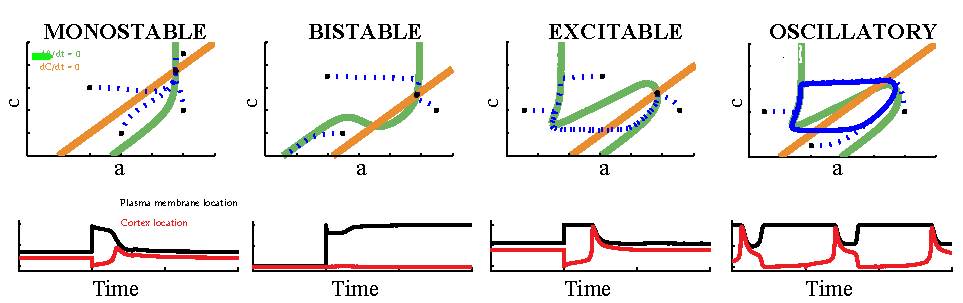
\includegraphics[width=4.5in]{Project2/figs/ODE_Analysis.pdf}
\caption{odes.}
\label{fig::odeanal}
\end{figure}

\begin{figure}[h]
\centering
\captionsetup{width=\linewidth}
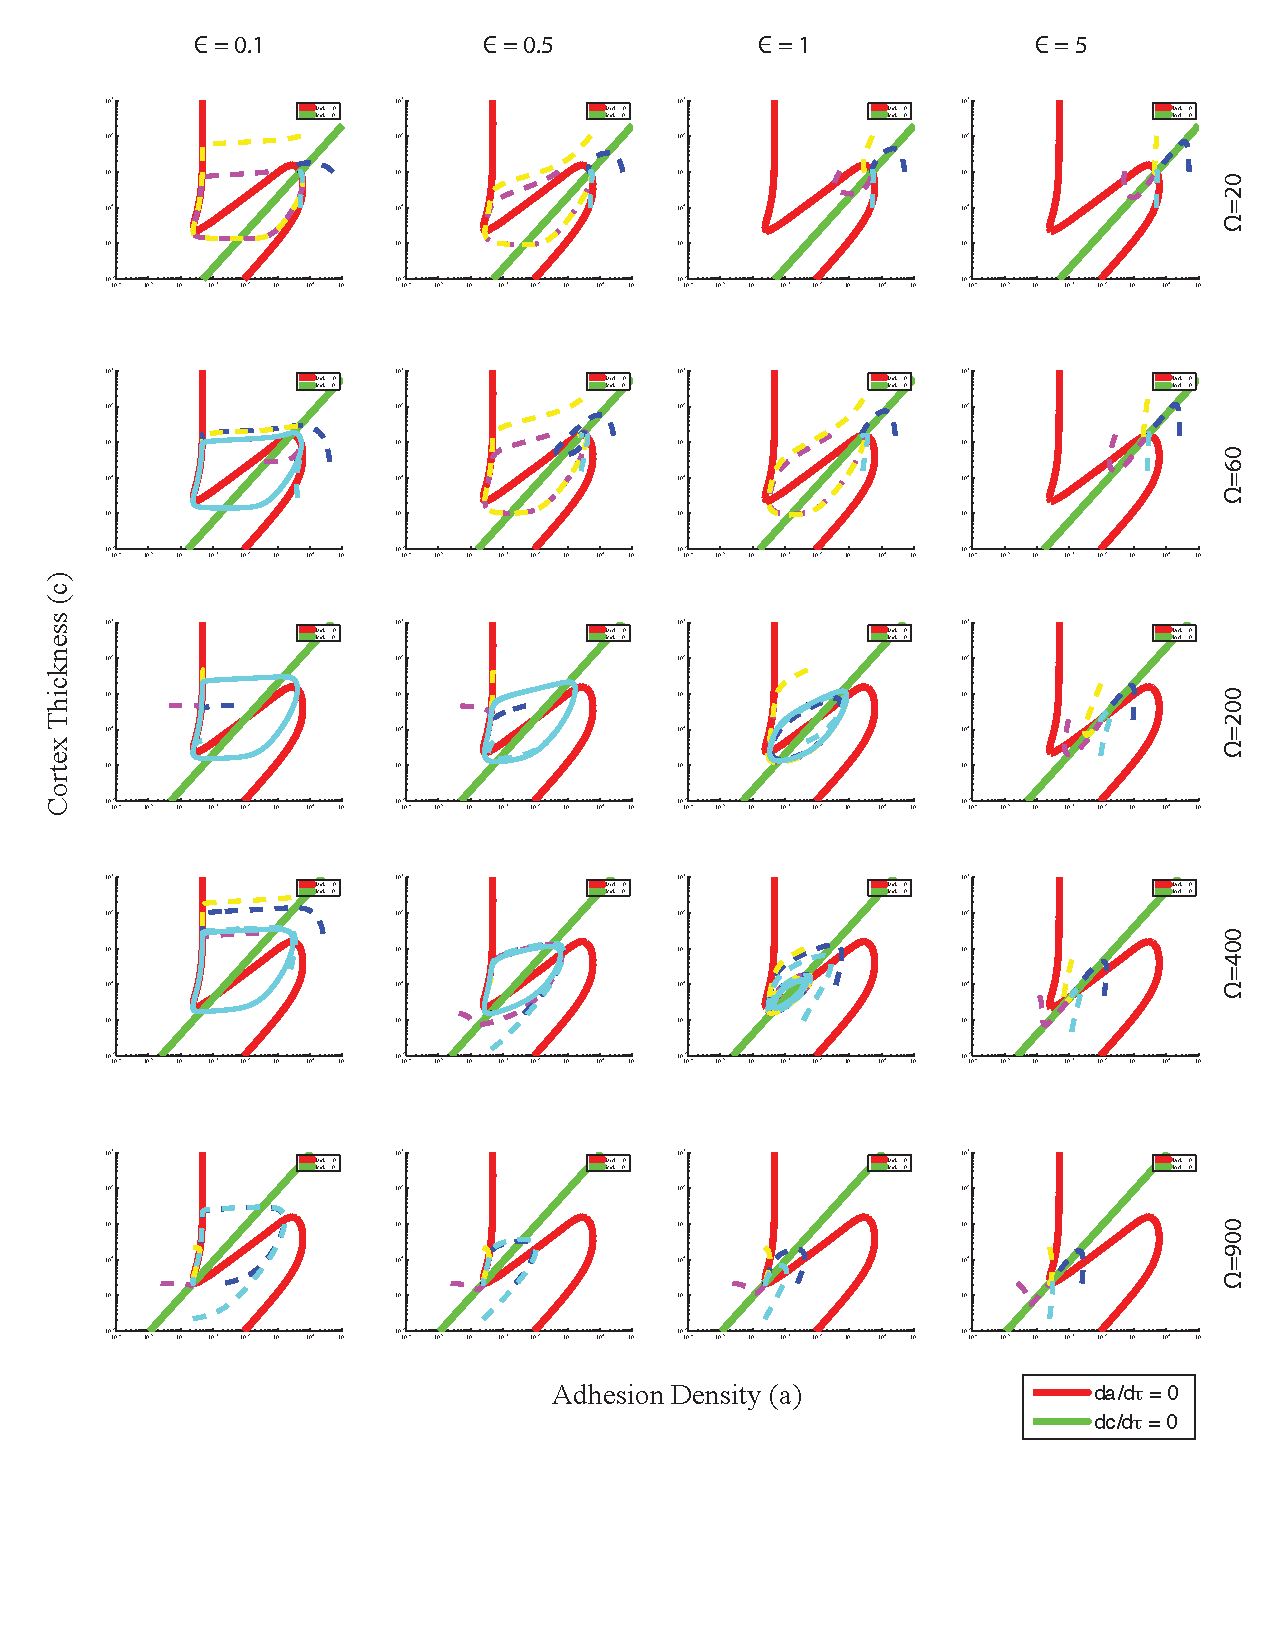
\includegraphics[width=4.5in]{Project2/figs/Epislon_omega.pdf}
\caption{two parameter bif.}
\label{fig::epsomega}
\end{figure}


\begin{figure}[h]
\centering
\captionsetup{width=\linewidth}
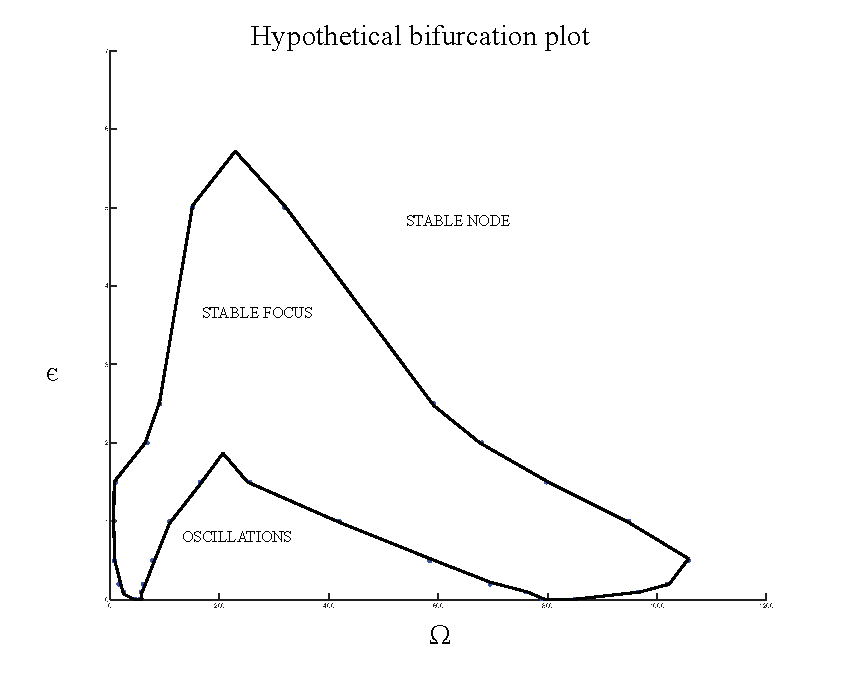
\includegraphics[width=4.5in]{Project2/figs/Hypothetical_bifurcation_plot.pdf}
\caption{two parameter bif.}
\label{fig::bifplot}
\end{figure}


\begin{figure}[h]
\centering
\captionsetup{width=\linewidth}
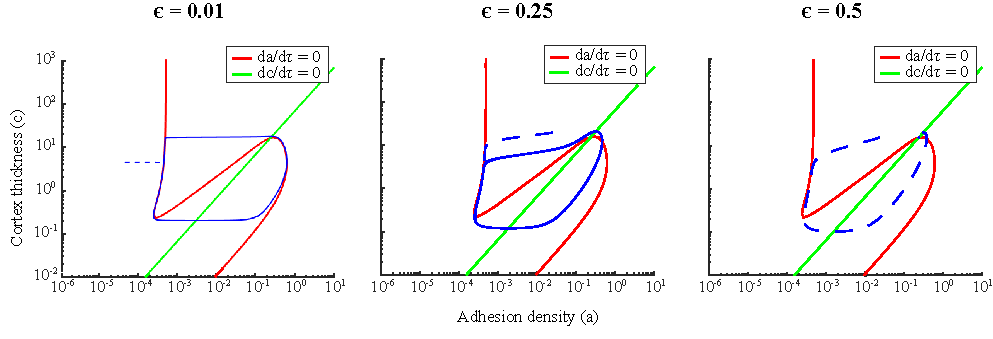
\includegraphics[width=4.5in]{Project2/figs/canard.pdf}
\caption{Canard.}
\label{fig::canard}
\end{figure}